%Summary here
The system evaluation complements the system implementation by measuring the performance of the developed solution, answering RQ2. This evaluation process will be carried out following a sequential approach.

This section details the research paradigm, the method, and the principles that will be used to carry out the system evaluation process, measuring the performance (latency, measured in seconds, and throughput, measured in rows/second) of reading and writing on Delta Lake or Apache Hudi while on \gls{HopsFS} of the current legacy pipeline and Rust-based pipelines. 

\subsection{Research paradigm}
The research paradigm for the system evaluation section of this thesis is more hybrid between positivism and post-positivism. While still performing a confirmatory research approach based on defined objectives, it considers the limitations and biases of this approach, not seeking to generalize the results obtained to other cases. This approach is motivated by the limitations and biases given by the industrial context of this thesis while performing a confirmatory analysis based on a newly implemented system.

\subsection{Evaluation process}
\label{subsec:eval_process}
The evaluation process will follow a sequential approach described in Figure \ref{fig:DevProcessRQ2}. Each step of this process is related to one of the goals (G5-G8) associated with the RQ2 in Section \ref{sec:goals}.
The relationship between each activity and the associated goal(s) is here explained:
\begin{enumerate}
    \item \textbf{Design experiments}: this activity maps perfectly to G5, designing the experiments that will be conducted to evaluate the performance difference in performance between the current legacy access to Apache Hudi compared to the delta-rs library-based access to Delta Lake in \gls{HopsFS}. 
    \item \textbf{Perform experiments}: this activity maps perfectly to G6, using the code implementation (D1) to conduct the designed experiments on the analyzed systems. Here, data is collected as latency, which is expressed in seconds.
    \item \textbf{Transform data according to metrics}: this activity is requisite to fulfill G7, as throughput is computed from latency and not measured. The relationship that relates throughput (rows/second), latency(seconds), and size of table (rows) is the following:
    \[ throughput \; (rows/second) = \frac{number \; of \; rows \; (rows)}{latency \;(seconds)}\]
    \item \textbf{Visualize results}: this activity maps perfectly to G7, visualizing the experiments' result according to two metrics, i.e., latency measured in seconds and throughput measured in rows/second. This activity also generates a deliverable (D2) of the experiment results complete with tables and histograms, i.e., Chapter \ref{ch:results_and_analysis}.
    \item \textbf{Analyze results}: this activity maps perfectly to G8, analyzing and interpreting the results delivered in D2. This deliverable contributes to D3, generating the analysis of results, i.e., Chapter \ref{ch:results_and_analysis}.
\end{enumerate}
\begin{figure}[!ht]
    \begin{center}
      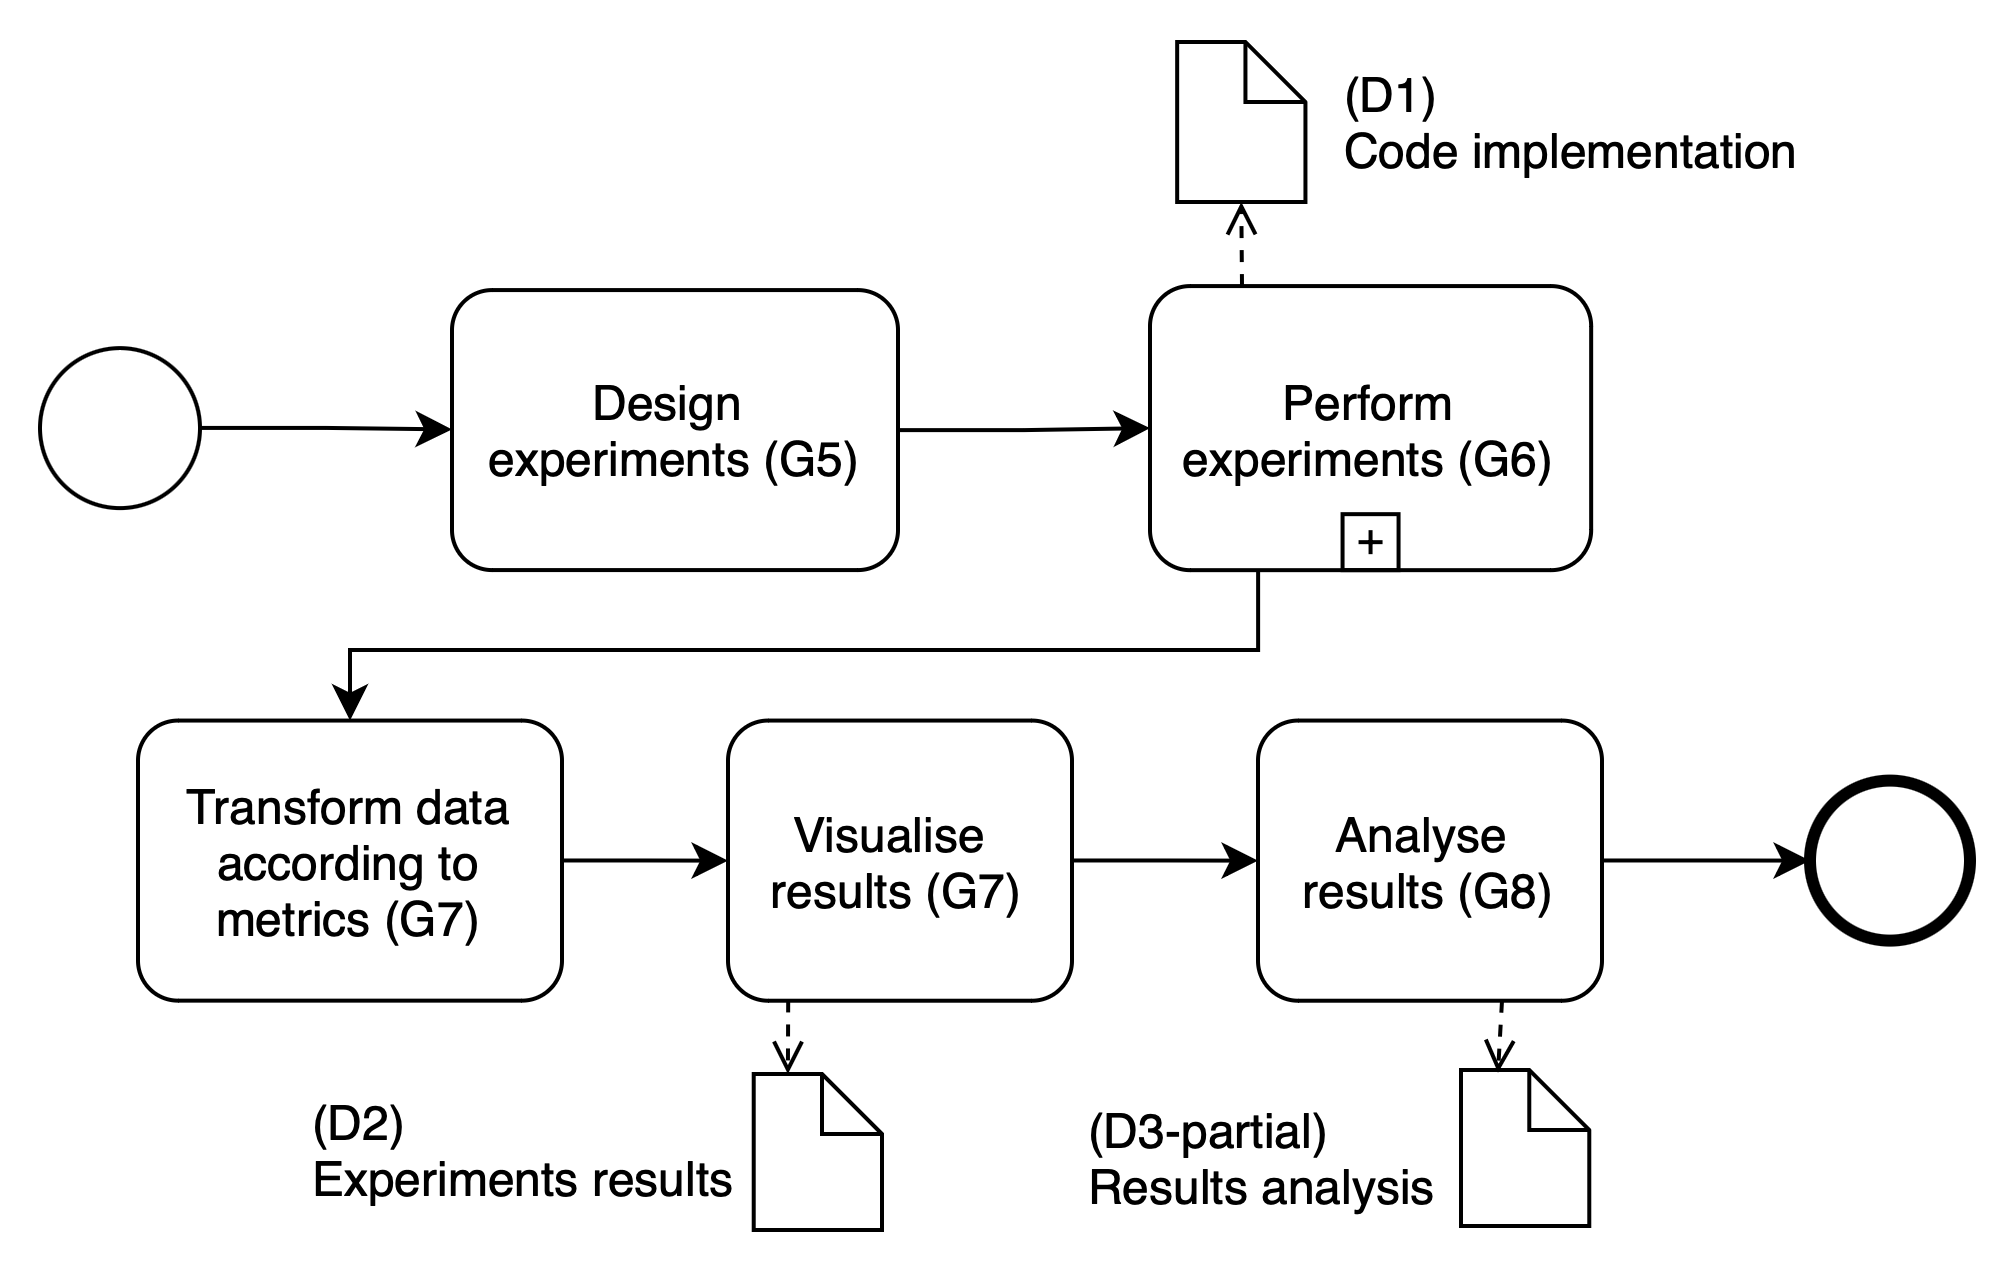
\includegraphics[width=\textwidth]{figures/3-method/research_process_rq2.png}
    \caption[System evaluation process]{\gls{BPMN} diagram of the System evaluation process answering to RQ2. Each activity is associated with a specific goal (\gls{G}). The process produces two deliverables (\gls{D}), the experiments results (D2) and a results analysis (D3-partial).}
    \label{fig:DevProcessRQ2}
    \end{center}
\end{figure}

\subsection{Industrial use case}
\label{subsec:use_case}

Several choices must be made for the system evaluation: which data will be used, which environment will run the experiments, and which metrics will be used to evaluate the system. While the other sections of this chapter detail which decisions were made, this section aims to outline a typical use case of the system implementation that can motivate the choices about how the system is going to be evaluated.

During the research work in Hopsworks \gls{AB}, the author talked to various employees and formed an idea of a typical client use case for the Hopsworks feature store. While these parameters are qualitative, they depict a specific use case around which this thesis work was built. Here below are these use case characteristics:
\begin{itemize}
  \item \textbf{Usage of rows over storage size}: contrary to Chapter \ref{ch:introduction}, where the size of workload is mainly referred to by storage size (bytes), in the experimental part of the thesis, only the number of rows will be used to refer to size. This choice is motivated by the need to find a reliable unit that measures a table size. Storage (bytes) is not strictly linked to a table structure (a table could have a lot of columns and a small number of rows and occupy the same memory as a table with a lot of rows but few columns), and it varies across storage structures (row-oriented format vs. column-oriented format, i.e., csv vs. parquet). Thus, storage size (bytes) alone is unreliable and cannot be used to measure data pipeline performance. This thesis kept the number of rows as the main unit to measure data size. Still, this metric was supplemented by specifying the number of columns and the data types in each row in Section \ref{subsec:data}.
  \item \textbf{Table size}: within Hopsworks, the author had the chance to see that most of the company's clients' workloads were limited (from 1M to 100M rows), while few clients had massive workloads (more than 1 BN rows). Given this outlook, this project opted to improve performance for the smaller workloads, setting the table sizes between 100K and 60M rows. The data selected is further detailed in Section \ref{subsec:data}.
  \item \textbf{Type of data}: the Hopsworks feature store works only with structured data (e.g., numbers, strings), and not with unstructured data (e.g., images, videos, audio) so, also the selected dataset in Section \ref{subsec:data} will reflect this scenario.
  \item \textbf{Client configuration}: the performance of the implemented system also depends on the computational and storage resources available on the client configuration running the system. The client configuration
  was modeled to reflect a limited number of setups. Four \gls{CPU} configurations were selected: one core, two cores, four cores, and eight cores. As for \gls{RAM} availability, this will be adapted to the system's needs (as it is unknown before running the experiments). Additionally, to avoid storage I/O bottlenecks and reflect a modern system, a system equipped with a \gls{SSD} storage will be used. The experimental environment is further detailed in Section \ref{subsec:exp_env}.
\end{itemize}

\subsection{Data}
\label{subsec:data}

The data that will be used to perform the read and write operations comes from \glsentryshort{TPC}-H benchmark suite~\footnote{Benchmark suite website available at \url{https://www.tpc.org/tpch/}}. \glsentryshort{TPC}-H is a decision support benchmark by \gls{TPC}. It consists of a series of business-oriented ad-hoc queries designed to be industry-relevant \cite{transactionprocessingperformancecounciltpcTPCH_v301pdf1993}. The data coming from this benchmark suite was used as
it provides a recognized standard for data storage systems \cite{TPC_benchmarks_2000}, and it has already been used in similar related work \cite{raasveldtDuckDBEmbeddableAnalytical2019, behmPhotonFastQuery2022}. Any part of the data can be generated using the TPC-H data generation tool~\footnote{Available at \url{https://www.tpc.org/tpc_documents_current_versions/current_specifications5.asp}}.

The \glsentryshort{TPC}-H benchmark contains eight tables. Of these two, SUPPLIER and LINEITEM were selected for the following reasons. The two tables are, respectively, the smallest (10000 rows) and largest (6000000 rows) tables whose size (number of rows) depends on the \gls{SF}. The \gls{SF} can be varied to obtain tables of different sizes (number of rows), allowing a progressive change in the table size (number of rows). 

The SUPPLIER table has seven columns, while the LINEITEM table has sixteen. This difference influences the average size of memory each row occupies. Below for each table their columns are listed, specifying which data type they store.
\begin{itemize}
  \item SUPPLIER
  \begin{itemize}
    \item S\_SUPPKEY : identifier
    \item S\_NAME : fixed text, size 25
    \item S\_ADDRESS : variable text, size 40
    \item S\_NATIONKEY : identifier
    \item S\_PHONE : fixed text, size 15
    \item S\_ACCTBAL : decimal
    \item S\_COMMENT : variable text, size 101
  \end{itemize}
  \item LINEITEM
  \begin{itemize}
    \item L\_ORDERKEY : identifier
    \item L\_PARTKEY : identifier
    \item L\_SUPPKEY : identifier
    \item L\_LINENUMBER : integer
    \item L\_QUANTITY : decimal
    \item L\_EXTENDEDPRICE : decimal
    \item L\_DISCOUNT : decimal
    \item L\_TAX : decimal
    \item L\_RETURNFLAG : fixed text, size 1
    \item L\_LINESTATUS : fixed text, size 1
    \item L\_SHIPDATE : date
    \item L\_COMMITDATE : date
    \item L\_RECEIPTDATE : date
    \item L\_SHIPINSTRUCT : fixed text, size 25
    \item L\_SHIPMODE : fixed text, size 10
    \item L\_COMMENT : variable text, size 44
  \end{itemize} 
\end{itemize}
As mentioned in Section \ref{subsec:use_case}, measuring the memory size in terms of bytes that a row of a table occupies has no single approach, as it depends on how the row is stored (e.g., a \gls{DBMS}, a row or column-oriented format). This limitation is why no specific ratio between a row and a data size in terms of bytes is given. Nonetheless, this section provides all information on the data, from how to retrieve it and how it is composed. These details enable the reader to calculate the storage occupancy of each table depending on its storage of choice.

Considering the different number of columns of the two tables used, the selected metrics, i.e., latency (seconds) and throughput(rows/second), cannot be used to compare results across different tables. This is why the comparative evaluation only considers different configurations on the same table.

This project used five table variations to benchmark the code solution as D1. \gls{SF} was varied to obtain a table at each significant figure, from 10000 rows to 60000000 rows. These are the tables:
\begin{enumerate}
    \item \textit{supplier\_sf1}: size = 10000 rows
    \item \textit{supplier\_sf10}: size = 100000 rows
    \item \textit{supplier\_sf100}: size = 1000000 rows
    \item \textit{lineitem\_sf1}: size = 60000000 rows
    \item \textit{lineitem\_sf10}: size = 60000000 rows
\end{enumerate}

\subsection{Experimental design}
\label{subsec:experimental_design}
% Description of which benchmarks will be performed and how. Here it needs to be explained the environment where the benchmarks will be run (Snurran), which tests are run, and why in this particular way.
%
% Talk about the selection of the questions: How do the performances vary if: (1) the newly implemented pipeline is used vs. the old pipeline. (2) a simple local filesystem implementation is used vs. writing on \gls{HopsFS} (3) varying the CPU configuration (4) we have different table sizes. 

The experiments aim to highlight the differences between the newly implemented system based on the delta-rs library and the current legacy system. Three different experimental pipelines were designed to isolate the benefit of using delta-rs over Spark and provide a baseline:
\begin{enumerate}
    \item \textbf{delta-rs - \glsentryshort{HopsFS}}: the system implemented in Chapter \ref{ch:implementation}. It comprises a Rust pipeline with Python bindings, enabling performing operations (i.e., reading, writing) on Delta Lake tables. This pipeline writes on \gls{HopsFS}.
    \item \textbf{delta-rs - \glsentryshort{LocalFS}}: this pipeline uses the same library as the system implemented but saves data on the \gls{LocalFS}. This pipeline provides a comparison within the delta-rs library, isolating the impact on performance caused by writing on \gls{HopsFS}, a distributed file system.
    \item \textbf{Legacy pipeline}: is the Hopsworks feature store which writes data on Hudi tables. This system uses a pipeline based on Kafka and Spark to write data on the Hudi tables, saved on \gls{HopsFS}. The pipeline uses a Spark alternative, DuckDB, and Arrow Flight to read data as explained in Section \ref{subsec:legacy_sys_reading}. 
\end{enumerate}

Furthermore, the experiments will verify how the performances of the three systems will change based on the \gls{CPU} resources provided: one core, two cores, four cores, or eight cores. Each time, the experimental environment will be modified, creating a new Jupyter server where the experiments will run with increasingly more resources. These \gls{CPU} configurations were chosen together with the industrial supervisor, according to the typical Hopsworks use case (Section \ref{subsec:use_case}). The data used for experiments, as described in Section \ref{subsec:data}, will come from two different tables. These are modified according to a \gls{SF}, for a total of five times. 

Additionally, during the writing experiments performed using the legacy pipeline, the contribution of different parts of the process will be measured, namely the upload time and materialization time, dichotomy explained in Section \ref{subsec:legacy_sys_writing}. This measurement will verify how different parts of the legacy pipeline scaled with table sizes and if Spark was the bottleneck of the architecture.

The Apache Hudi pipelines are preferred over the new Spark-based pipeline reading and writing on Delta Lake because they were released and tested extensively on the Hopsworks platform, so they provide more guarantees of obtaining relevant results. Additionally, at the time of experiment design, these two variations, Spark writing on Delta Lake and Spark writing on Apache Hudi, were considered similarly in read and write performance. 

In conclusion, the experiments conducted will be a total of three (pipelines) times four (\gls{CPU} configurations) times five (tables) times two (read and write operations), i.e., one hundred and twenty experiments, performed fifty times each to create statistically significant results.

\subsection{Experimental environment}
\label{subsec:exp_env}
% Describe Snurran

The experimental environment consists of a physical machine in Hopsworks' offices, which is virtualized to enable remote shared development. The \gls{CPU} details of the machine are present in Listing \ref{lst:cpu_snurran}, noting that only eight cores at maximum were accessed during the experiments. It should be observed that this experimental environment, while virtualized in isolation, runs on shared computing resources, so experiment results might vary depending on the machine's load. Considering this, all experiments will be run when the machine load is low (less than 50\% of \gls{CPU} and \gls{RAM} usage) to limit having results depending on external workloads running.

The machine mounts about 5.4 TBs of \gls{SSD} memory. This storage allows the machine to have fast read and write speed, 2.7 GB/s, and 1.9 GB/s, respectively (measured with a simple \textit{dd} bash command). 

The experimental environment will be set up with a Jupyter Server of different CPU cores, depending on the experiment. The Jupyter server is allocated by default with 2048 MB of \gls{RAM} out of the 192 GB  available on the experimental machine. This amount will be adjusted during the experiments according to the needs of the experiments (see Section \ref{subsec:resources_usage}).

\begin{lstlisting}[language=bash, caption={[Experimental environment details]Output of a \textit{lscpu} bash command in the experimental environment.}, label={lst:cpu_snurran}, frame=tb]
Architecture:            x86_64
  CPU op-mode(s):        32-bit, 64-bit
  Address sizes:         48 bits physical, 
                         48 bits virtual
  Byte Order:            Little Endian
CPU(s):                  32
  On-line CPU(s) list:   0-31
Vendor ID:               AuthenticAMD
  Model name:            AMD Ryzen Threadripper 
                         PRO 5955WX 16-Cores
    CPU family:          25
    Model:               8
    Thread(s) per core:  2
    Core(s) per socket:  16
    Socket(s):           1
    Stepping:            2
    Frequency boost:     enabled
    CPU max MHz:         7031.2500
    CPU min MHz:         1800.0000
    BogoMIPS:            7985.56
Virtualization features: 
  Virtualization:        AMD-V
Caches (sum of all):     
  L1d:                   512 KiB (16 instances)
  L1i:                   512 KiB (16 instances)
  L2:                    8 MiB (16 instances)
  L3:                    64 MiB (2 instances)
\end{lstlisting}

\subsection{Evaluation framework}
% Describe which metrics are used to evaluate the system. Which metrics were used during the experiments
%
% What I would like to say is essentially that:
% This evaluation section's objective is to: Verify The system requirements defined in ... , and compare the performance (defined as throughput in RQ2) with older systems. Explain how both of these things are done.

The system evaluation framework is designed to evaluate three key aspects of the system using different metrics:
\begin{enumerate}
    \item \textbf{Functional requirements}: defined in Section \ref{subsec:requirements}, functional requirements will be measured by verifying the success or failure of running an experiment. This will not happen by design, as the system implementation phase continues until all functional requirements are met.
    \item \textbf{Non-functional requirements}: defined in Section \ref{subsec:requirements}, non-functional requirements are: consistency, maintainability and scalability. The first two requirements are mainly addressed during implementation, while scalability is measured during the system evaluation experiments. The metric used for measuring this requirement is the throughput measured in rows/second, as defined in RQ2.
    \item \textbf{How does the legacy system compare to other pipelines?}: this question answers directly RQ2, measuring the throughput measured in rows/second of the different pipelines, defined in Section \ref{subsec:experimental_design}. Results are then compared using a visual approach.
\end{enumerate} 

\subsection{Assessing reliability and validity}
\label{subsec:reliability_validity}
% Here explain how the readability and validity of the collected data were addressed. Mainly here the bootstrapping method needs to explained and how it achieves getting a CI without making assumption on the data distribution.

Results are significant according to their reliability and validity. In this project work, each experiment will be performed fifty times to ensure the reliability of the experiment results on the system performance. This number was agreed to balance the results' consistency and the limited resources available (in terms of time and computing resources).

Due to the complex nature of the pipelines used, the data distribution of results could vary from one experiment to the other. This hampers the possibility of comparing results, significantly impacting the relevance of the results analysis. A bootstrapping technique will be used to restore the validity of the data collected. Data will be resampled with substitution a thousand times, then an average with a confidence interval for each experiment will be calculated. This will benefit the accuracy of the results presented.